\section{Showcase of the Project}
\label{sec:showcase-of-the-project}

\hspace{1cm} Having gone through the recondite details of the implementation, including the used libraries, the precompiled header for efficient compilation, the Makefile for manageable builds, and the core game logic, the game GUI loop, we now come to the Showcase section. Here we will show the practical application of our poker game in respect to key features, gameplay mechanics, and user interface. The following sections will provide a detailed walkthrough of entire game. You can rather watch the video of the game showcase via this \href{https://youtu.be/OA0v6xG21N4}{YouTube link}.

\subsection{Start Screen}

\begin{figure}[H]
    \centering
    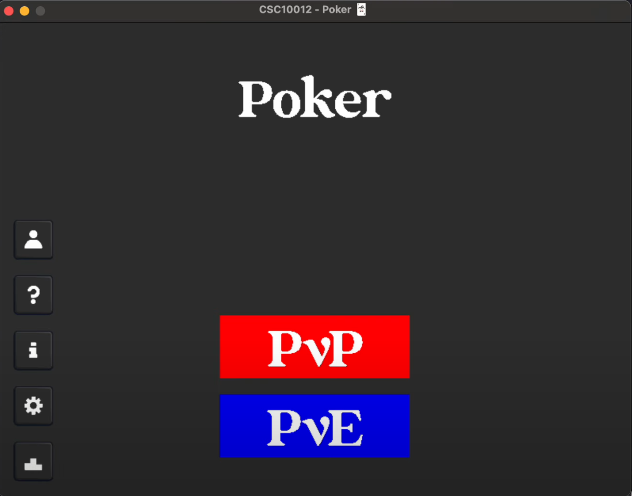
\includegraphics[width=0.7\textwidth]{figures/start_screen.png}
    \caption{Start Screen}
    \label{fig:start-screen}
\end{figure}

\hspace{1cm} The game starts with no loading screen, directly to the start screen. The start screen is simple and clean, with the game title at the top, and 5 buttons at the bottom left corner and 2 buttons at the bottom middle of the screen, each with a different function. The buttons are: 

\begin{enumerate}
    \item \textbf{User Info}: The button that has the icon of a person.
    \\ This button navigate the user to the login screen, where they can login or register a new account. You can view the login screen in \hyperref[subsec:login-screen]{Login Screen} section.
    \item \textbf{Tutorial}: The button that has the icon of a question mark.
    \\ This button navigate the user to the tutorial screen, where they can learn about the ranking of the poker hands. You can view the tutorial screen in \hyperref[subsec:tutorial-screen]{Tutorial Screen} section.
    \item \textbf{About Us}: The button that has the icon of the character "i", which stands for information.
    \\ This button navigate the user to the about us screen, where they can learn about us - the developers of this game. You can view the tutorial screen in \hyperref[subsec:about-us-screen]{About Us Screen} section.
    \item \textbf{Settings}: The button that has the icon of a gear.
    \\ This button navigate the user to the settings screen, where they can change the settings of the game, such as the background music, the sound effects, and the game mode. You can view the tutorial screen in \hyperref[subsec:settings-screen]{Settings Screen} section.
    \item \textbf{Leaderboard}: The button that has the icon of a standing podium.
    \\ This button navigate the user to the leaderboard screen, where they can view all the players and their corresponding information.
    \item \textbf{PvP}: The button that has the text "PvP" on it.
    \\ This button navigate the user to the PvP screen, based on the current game mode, the user can play either Basic Poker or Draw Poker.
    \item \textbf{PvE}: The button that has the text "PvE" on it.
    \\ This button navigate the user to the PvE screen, where the user can play Basic Poker against 5 computer players.
\end{enumerate}

\subsection{Login Screen}
\label{subsec:login-screen}

\begin{figure}[H]
    \centering
    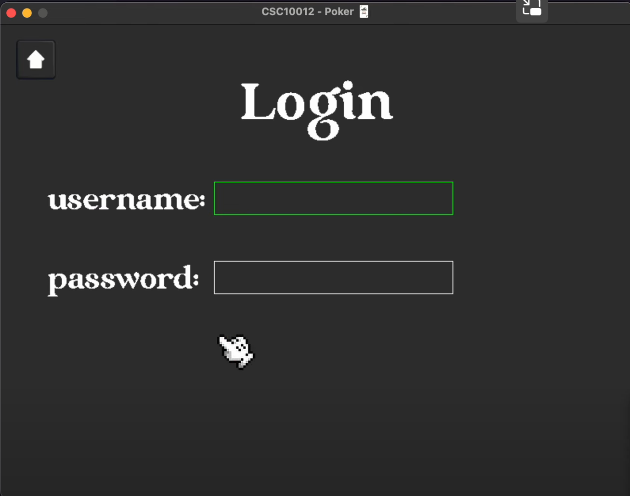
\includegraphics[width=0.7\textwidth]{figures/login_screen.png}
    \caption{Login Screen}
    \label{fig:login-screen}
\end{figure}

\hspace{1cm} The login screen is simple and clean, with the title of the screen at the top, and 2 text fields for the user to input their username and password, one downside of the screen is that user need to use \texttt{tab} key to navigate between the text fields, we have not implemented the mouse click to navigate between the text fields yet. When there is a new username, a prompt will appear to ask the user to register a new account. If the user has an existing account, they can login by inputting their username and password, then press \texttt{enter} key to login to the game. A small status message will appear at the bottom middle of the screen to inform the user about the status of their login process whether it is successful or it is an incorrect username or password. The user can navigate back to the start screen by pressing the back button at the top left corner of the screen, the button that has the icon of a house.

\vspace{0.5cm}

\hspace{1cm} You can view the demonstration video of the login screen via this \href{https://youtu.be/OA0v6xG21N4?t=165}{YouTube timestamp link}.

\subsection{Tutorial Screen}
\label{subsec:tutorial-screen}

\begin{figure}[H]
    \centering
    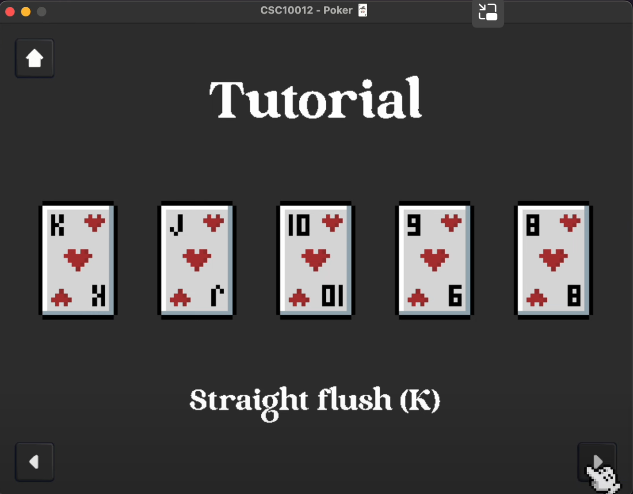
\includegraphics[width=0.7\textwidth]{figures/tutorial_screen.png}
    \caption{Tutorial Screen}
    \label{fig:tutorial-screen}
\end{figure}

\hspace{1cm} The tutorial screen is simple and intuitive, with the title of the screen at the top, and the content of the tutorial in the middle of the screen. At the bottom left corner of the screen, there is a back button that has the icon of a left arrow, which allows the user to navigate back to the previous demonstration of a hand ranking in Poker. At the bottom right corner of the screen, there is a next button that has the icon of a right arrow, which allows the user to navigate to the next demonstration of a hand ranking in Poker. The user can navigate back to the start screen by pressing the back button at the top left corner of the screen, the button that has the icon of a house. Also at the bottom middle of the screen, there is a status message that informs the user about the current demonstration of the hand they are viewing.

\vspace{0.5cm}

\hspace{1cm} You can view the demonstration video of the tutorial screen via this \href{https://youtu.be/OA0v6xG21N4?t=120}{YouTube timestamp link}.

\subsection{About Us Screen}
\label{subsec:about-us-screen}

\hspace{1cm} Unfortunately, we have not implemented the about us screen yet. The about us screen will contain information about us - the developers of this game, but we think that it is not necessary to implement this feature at the moment. We will consider implementing this feature in the future if we have time.

\subsection{Settings Screen}
\label{subsec:settings-screen}

\begin{figure}[H]
    \centering
    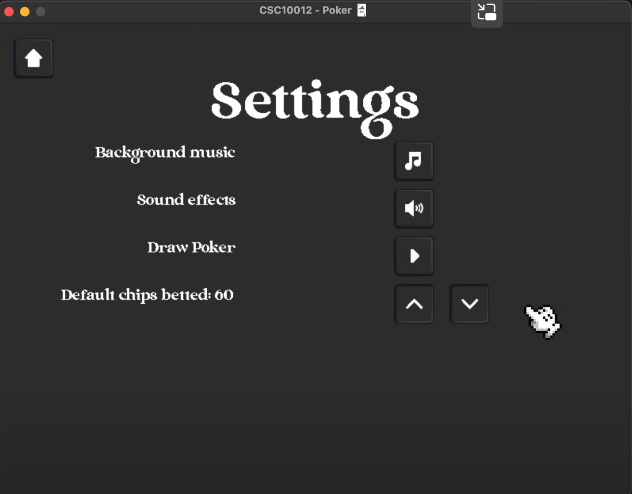
\includegraphics[width=0.7\textwidth]{figures/settings_screen.png}
    \caption{Settings Screen}
    \label{fig:settings-screen}
\end{figure}

\hspace{1cm} The settings screen is simple, with the title of the screen at the top, and 4 rows of settings that the user can change. The user can navigate back to the start screen by pressing the back button at the top left corner of the screen, the button that has the icon of a house. The 4 rows of settings are:
\begin{enumerate}
    \item \textbf{Background Music}: The first row of settings is the background music, where the user can turn on or off the background music. The user can change the background music by pressing the music note icon on the right side of the row. Notice that the background music will be turned on by default when the user starts the game. And the button will change its texture to indicate the current status of the background music.
    \item \textbf{Sound Effects}: The second row of settings is the sound effects, where the user can turn on or off the sound effects. The user can change the sound effects by pressing the sound icon on the right side of the row. And the button will change its texture to indicate the current status of the sound effects.
    \item \textbf{Game Mode}: The third row of settings is the game mode, where the user can change the game mode to either Basic Poker or Draw Poker. The user can change the game mode by pressing the right arrow icon on the right side of the row.
    \item \textbf{Default entry fee (chips)}: The fourth row of settings is the default entry fee, where the user can change the default entry fee to play the game. The user can change the default entry fee by pressing the up or down arrow icon on the right side of the row. When pressing the up arrow icon, the default entry fee will increase by 20 chips, and when pressing the down arrow icon, the default entry fee will decrease by 20 chips.
\end{enumerate}

\hspace{1cm} You can view the demonstration video of the settings screen via this \href{https://youtu.be/OA0v6xG21N4?t=144}{YouTube timestamp link}.

\subsection{Leaderboard Screen}
\label{subsec:leaderboard-screen}

\begin{figure}[H]
    \centering
    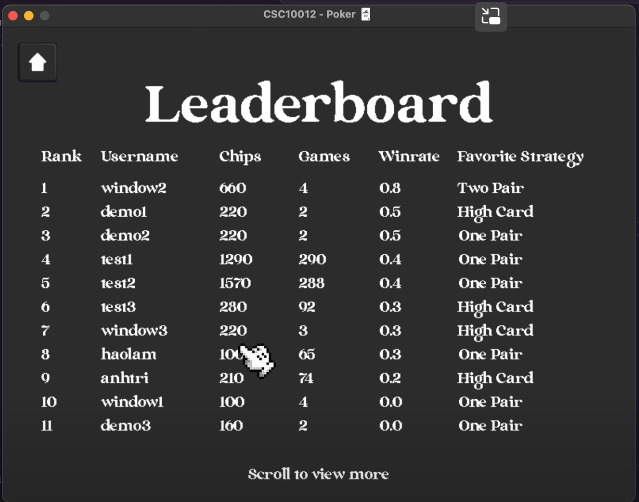
\includegraphics[width=0.7\textwidth]{figures/leaderboard_screen.png}
    \caption{Leaderboard Screen}
    \label{fig:leaderboard-screen}
\end{figure}

\hspace{1cm} In the leaderboard screen, the user can view all the registered players and their corresponding information such as their rank, username, chips, number of played games, winrate and their favorite strategy. The user can navigate back to the start screen by pressing the back button at the top left corner of the screen, the button that has the icon of a house. In this screen, if there are more than 11 players, the user can scroll through the leaderboard by using the mouse wheel.

\vspace{0.5cm}

\hspace{1cm} You can view the demonstration video of the leaderboard screen via this \href{https://youtu.be/OA0v6xG21N4?t=302}{YouTube timestamp link}.

\subsection{PvP Screen}
\label{subsec:pvp-screen}

\begin{figure}[H]
    \centering
    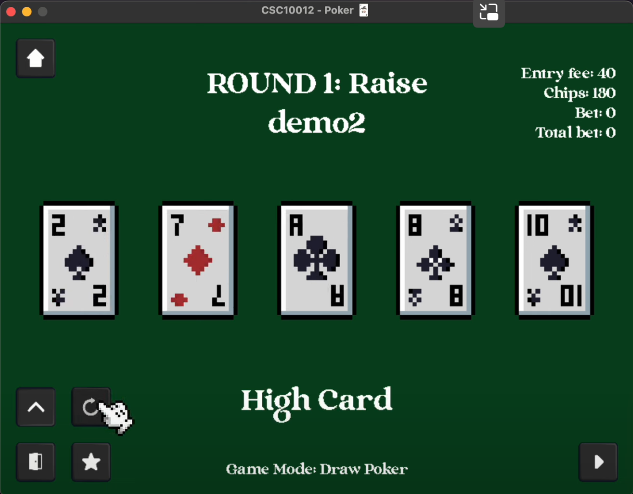
\includegraphics[width=0.7\textwidth]{figures/pvp_screen.png}
    \caption{PvP Screen}
    \label{fig:pvp-screen}
\end{figure}

\hspace{1cm} The PvP screen is one of the core features of the game, where the user can play against another player in real-time. This screen will change its render logic based on the current game mode.

\vspace{0.5cm}

\hspace{1cm} For Basic Poker game mode, the screen will display each of the player's hand and their corresponding information such as their username, chips, and their current bet. The user can click on their card to reveal the card, and click on the card again to hide the card, that's it. When all the cards facing up, a small status message will appear at the bottom middle of the screen to inform the user about the hand ranking of the player. After viewing their card, the user can click on the next button to proceed to the next player. When click that button, all of the cards of the next player will be faced down and the next player can now go to the computer and view their card. This process will repeat until all of the players have viewed their card. After that, the game will proceed to the result screen, where the winner will be announced and their card will be revealed for all the players to see.

\vspace{0.5cm}

\hspace{1cm} For Draw Poker game mode, the screen will display each of the player's hand and their corresponding information such as their username, chips, and their current bet just like the basic poker game mode. The difference here is that now the player have to deal with 4 new buttons, which are the call, raise, fold, and draw button. Here come the new mechanics of the game:
\begin{enumerate}
    \item \textbf{Call}: The call button allows the player to match the current highest bet of the game. The player can only call if they have enough chips to match the current highest bet.
    \item \textbf{Raise}: The raise button allows the player to raise their own bet, each time the player press that button, their own bet will increase by 20 chips. The player can only raise if they have enough chips to raise their own bet.
    \item \textbf{Fold}: The fold button allows the player to fold their hand, which means they will lose the current game and their bet will be taken by the winner of the game.
    \item \textbf{Draw}: The draw button allows the player to draw new cards from the deck. We have implemented the right mouse click to select the card that the player wants to draw. The player can only choose up to 3 cards to draw, and they can only draw once. After the player has drawn the card, there is nothing left they can do, they should press the next button to proceed to the next player.
\end{enumerate}

\hspace{1cm} We also handle if that button can be clicked or not in the current round of the game. It should be cleaner if we manage to also fade out the button that cannot be clicked to have a better user experience. However, we think that it is not necessary to implement this feature at the moment. We will consider implementing this feature in the future.

\vspace{0.5cm}

\hspace{1cm} Finally, you can view the demonstration video of the PvP screen Draw Poker game mode via this \href{https://youtu.be/OA0v6xG21N4?t=308}{YouTube timestamp link}.

\subsection{PvE Screen}
\label{subsec:pve-screen}

\begin{figure}[H]
    \centering
    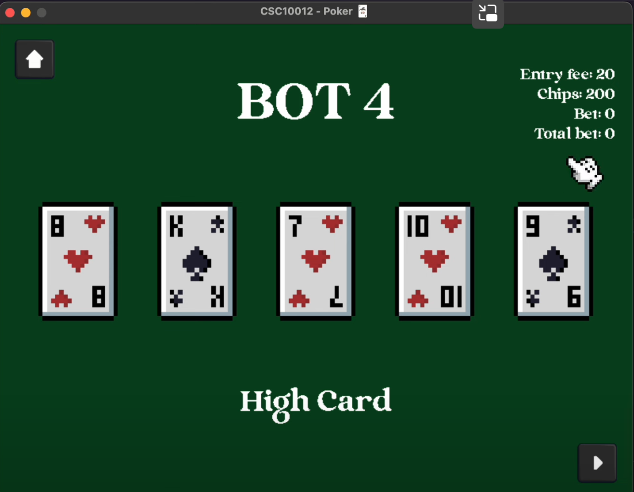
\includegraphics[width=0.7\textwidth]{figures/pve_screen.png}
    \caption{PvE Screen}
    \label{fig:pve-screen}
\end{figure}

\hspace{1cm} The PvE screen is one of the core features of the game, where the user can play against 5 computer players. This screen will not change its render logic based on the current game mode since we only support Basic Poker game mode for PvE screen. The screen will display each of the player's hand and their corresponding information such as their username, chips, and their current bet. The user can click on their card to reveal the card, and click on the card again to hide the card, that's it. When all the cards facing up, a small status message will appear at the bottom middle of the screen to inform the user about the hand ranking of the player. After viewing their card, the user can click on the next button to proceed to the next player. When click that button, all of the cards of the next player will be faced down and the next player can now go to the computer and view their card. It's just quite similar to the PvP screen, but the difference is that the user will play against 5 more bot players.

\vspace{0.5cm}

\hspace{1cm} Our bot players are quite simple, their cards will be facing up by the player click. Their information is also displayed on the screen, such as their username, chips, and their current bet. Notice that, if the player win against bots, they will not get any chips, but if they lose, they will lose the chips that they bet, since we want our game to be more challenging and closer to the real poker game where bots are quite hard to beat and have significant advantages over the player. We will consider implementing the reward system for the player if they win against bots in the future.

\vspace{0.5cm}

\hspace{1cm} Finally, you can view the demonstration video of the PvE screen via this \href{https://youtu.be/OA0v6xG21N4?t=210}{YouTube timestamp link}.

% ------------------- THE END ------------------- %